\documentclass[UTF8]{ctexart}
%%%%%%%%%%%%%%%%%%%%%%%%%%%== 引入宏 ==%%%%%%%%%%%%%%%%%%%%%%%%%%%%%
\usepackage{cite}
\usepackage{amsmath}	% 使用数学公式
\usepackage{graphicx}	% 插入图片/PDF/EPS 等图像
\usepackage{subfigure}	% 使用子图像或者子表格
\usepackage{geometry}	% 设置页边距
\usepackage{fancyhdr}	% 设置页眉页脚
\usepackage{setspace}	% 设置行间距
\usepackage{hyperref}	% 让生成的文章目录有链接,点击时会自动跳转到该章节
\usepackage{url}
\usepackage{caption2}
\usepackage{forest}
\usepackage{float}
\usepackage{listings}
\usepackage{listings-golang}
\usepackage{color} 

\setmonofont{Monaco}

\definecolor{mygreen}{rgb}{0,0.6,0}
\definecolor{mygray}{rgb}{0.5,0.5,0.5}
\definecolor{mymauve}{rgb}{0.58,0,0.82}
\lstset{ %
  backgroundcolor=\color{white},   % choose the background color
  basicstyle=\footnotesize\ttfamily,        % size of fonts used for the code
  columns=flexible,
  breaklines=true,                 % automatic line breaking only at whitespace
  captionpos=b,                    % sets the caption-position to bottom
  tabsize=4,
  commentstyle=\color{mygreen},    % comment style
  escapeinside={\%*}{*)},          % if you want to add LaTeX within your code
  keywordstyle=\color{blue},       % keyword style
  stringstyle=\color{mymauve}\ttfamily,     % string literal style
  frame=shadowbox,
  rulesepcolor=\color{mygray},
  language=Golang,
  xleftmargin=2em,
  xrightmargin=2em, 
  aboveskip=1em
}

\def\ojoin{\setbox0=\hbox{$\bowtie$}%
  \rule[-.02ex]{.25em}{.4pt}\llap{\rule[\ht0]{.25em}{.4pt}}}
\def\leftouterjoin{\mathbin{\ojoin\mkern-5.8mu\bowtie}}
\def\rightouterjoin{\mathbin{\bowtie\mkern-5.8mu\ojoin}}
\def\fullouterjoin{\mathbin{\ojoin\mkern-5.8mu\bowtie\mkern-5.8mu\ojoin}}

%%%%%%%%%%%%%%%%%%%%%%%%%%== 设置全局环境 ==%%%%%%%%%%%%%%%%%%%%%%%%%%%%
% [geometry] 设置页边距
\geometry{top=2.6cm, bottom=2.6cm, left=2.45cm, right=2.45cm, headsep=0.4cm, foot=1.12cm}
% 设置行间距为 1.5 倍行距
\onehalfspacing
% 设置页眉页脚
\pagestyle{fancy}
%\lhead{左头标}
%\chead{\today}
%\rhead{152xxxxxxxx}
\lfoot{}
\cfoot{\thepage}
\rfoot{}
%\renewcommand{\headrulewidth}{0.4pt}
%\renewcommand{\headwidth}{\textwidth}
%\renewcommand{\footrulewidth}{0pt}

%%%%%%%%%%%%%%%%%%%%%%%%%%== 自定义命令  ==%%%%%%%%%%%%%%%%%%%%%%%%%%%%%%
% 此行使文献引用以上标形式显示
\newcommand{\supercite}[1]{\textsuperscript{\cite{#1}}}
% 此行使section中的图、表、公式编号以A-B的形式显示
\renewcommand{\thetable}{\arabic{section}-\arabic{table}}
\renewcommand{\thefigure}{\arabic{section}-\arabic{figure}}
\renewcommand{\theequation}{\arabic{section}-\arabic{equation}}
% 此行使图注、表注与编号之间的分隔符缺省,默认是冒号:
\renewcommand{\captionlabeldelim}{~}

%===================================== 标题设置  ==========================================
% \heiti \kaishu 为字体设置,ctex 会自动根据操作系统加载字体
\title{\huge{\heiti Talent-Plan Section 4}}
\author{\small{\kaishu 宋阳}\\[2pt]
\small{\kaishu 北京航空航天大学}\\[2pt]
\small{Email:}
\url{yangsoonlx@gmail.com}
}
\date{} % 去除默认日期
%\date{\today}

%===================================== 正文区域  ==========================================
\begin{document}
\maketitle
% \tableofcontents % 目录内容,注释取消掉可实现目录

\begin{flushleft}
\textbf{课程目标}:熟悉数据库基础知识 \\[8pt]
\end{flushleft}
\section{课程作业}\label{sec1}	
用 Go 语言, 实现一个 Join 算法, 从两个 CSV 文件中读取数据,
在一个或多个等值条件上进行链接,并对最终结果求和。
请参考 README,使用提供的框架完成作业,并跑通测试程序。
提交的作业要求代码整洁规范,附有文档,并提供对程序的性能瓶颈分析及优化思路。 \\

\section{课程报告}\label{sec2}

\subsection{实验结果}
本次实验实现了两类解决方案,一个是从计算上进行优化,利用多核特征在probe阶段并行计算,
另一种实现是在从磁盘读取时,边读取边进行计算,做到IO任务和CPU任务重叠进行。第一种利用多核
特性的函数命名为$JoinBase$,第二种IO任务和CPU任务重叠的函数命名为$Join$,下面分别展示在小数据
和大数据的场景下的bench结果。

1. 第一种情况属于小数据量的场景, join时,左表为r0(107KB), 右表为r2(10KB),左表比右表大。
\begin{lstlisting}[language={bash}]
  go test -bench Benchmark -run xx -count 5 -benchmem
  goos: darwin
  goarch: amd64
  pkg: join
  BenchmarkJoinBase-4      	     451	   2573938 ns/op	 1672971 B/op	   21121 allocs/op
  ...
  BenchmarkJoinBase-4      	     460	   2836937 ns/op	 1672917 B/op	   21121 allocs/op
  BenchmarkJoin-4          	     502	   2411289 ns/op	 2869716 B/op	   21351 allocs/op
  ...
  BenchmarkJoin-4          	     480	   2356291 ns/op	 2869892 B/op	   21352 allocs/op
  BenchmarkJoinExample-4   	     304	   3877400 ns/op	 3676971 B/op	   21897 allocs/op
  ...
  BenchmarkJoinExample-4   	     307	   3784964 ns/op	 3677016 B/op	   21897 allocs/op
  PASS
  ok  	join	24.179s
\end{lstlisting}

2. 第二种情况也属于小数据量的场景, join时,左表为r2(10KB), 右表为r0(107KB),左表比右表小。
\begin{lstlisting}[language={bash}]
  go test -bench Benchmark -run xx -count 5 -benchmem
  goos: darwin
  goarch: amd64
  pkg: join
  BenchmarkJoinBase-4      	     442	   2510995 ns/op	 1689349 B/op	   21121 allocs/op
  ...
  BenchmarkJoinBase-4      	     471	   2425857 ns/op	 1689286 B/op	   21121 allocs/op
  BenchmarkJoin-4          	     589	   2141705 ns/op	  886498 B/op	   21097 allocs/op
  ...
  BenchmarkJoin-4          	     584	   1969355 ns/op	  886459 B/op	   21096 allocs/op
  BenchmarkJoinExample-4   	     429	   2720058 ns/op	 1769025 B/op	   31110 allocs/op
  ...
  BenchmarkJoinExample-4   	     433	   2729499 ns/op	 1768992 B/op	   31110 allocs/op
  PASS
  ok  	join	23.143s
\end{lstlisting}

3. 第三种情况属于较大数据量的场景, join时,左表为t0(212.6MB), 右表为t2(68.3MB),左表比右表大。
\begin{lstlisting}[language={bash}]
  go test -bench Benchmark -run xx -count 5 -benchmem
  goos: darwin
  goarch: amd64
  pkg: join
  BenchmarkJoinBase-4      	       1	6370735189 ns/op	2562076016 B/op	21603453 allocs/op
  ...
  BenchmarkJoinBase-4      	       1	5024537792 ns/op	2562070376 B/op	21603540 allocs/op
  BenchmarkJoin-4          	       1	3420110407 ns/op	2268295568 B/op	21914390 allocs/op
  ...
  BenchmarkJoin-4          	       1	3294719695 ns/op	2268229368 B/op	21913928 allocs/op
  BenchmarkJoinExample-4   	       1	8738835711 ns/op	3525159312 B/op	26919518 allocs/op
  ...
  BenchmarkJoinExample-4   	       1	8872588663 ns/op	3525079296 B/op	26918959 allocs/op
  PASS
  ok  	join	92.804s
\end{lstlisting}

4. 第四种情况也属于较大数据量的场景, join时,左表为t2(68.3MB), 右表为t0(212.6MB), 左表比右表小。
\begin{lstlisting}[language={bash}]
  go test -bench Benchmark -run xx -count 5 -benchmem
  goos: darwin
  pkg: join
  BenchmarkJoinBase-4      	       1	6073820292 ns/op	2747795416 B/op	21705016 allocs/op
  ...
  BenchmarkJoinBase-4      	       1	5674971829 ns/op	2747783840 B/op	21704950 allocs/op
  BenchmarkJoin-4          	       1	2799017553 ns/op	1555142400 B/op	21715882 allocs/op
  ...
  BenchmarkJoin-4          	       1	2859071642 ns/op	1555027776 B/op	21715088 allocs/op
  BenchmarkJoinExample-4   	       1	8102270767 ns/op	2913906920 B/op	34687841 allocs/op
  ...
  BenchmarkJoinExample-4   	       1	8302536321 ns/op	2913893216 B/op	34687747 allocs/op
  PASS
  ok  	join	85.728s
\end{lstlisting}

\subsection{实现和优化}
\subsubsection{利用多核特性的 $JoinBase$}
通过查看$JoinExample$的代码,我首先做了3个优化。
\begin{enumerate}
  \item 选择较小的关系表来产生hash结果。
  \item $JoinExample$里面对左表进行hash时,键值对中的值存储的是左表的下标地址。在$JoinBase$中当小表是左表时,
  我选择直接存储对应的row[0]值。
  \item 在join的probe阶段将大表根据核数进行切分,划分为多个goroutine并行计算。
\end{enumerate}
\begin{figure}[H]
  \centering
  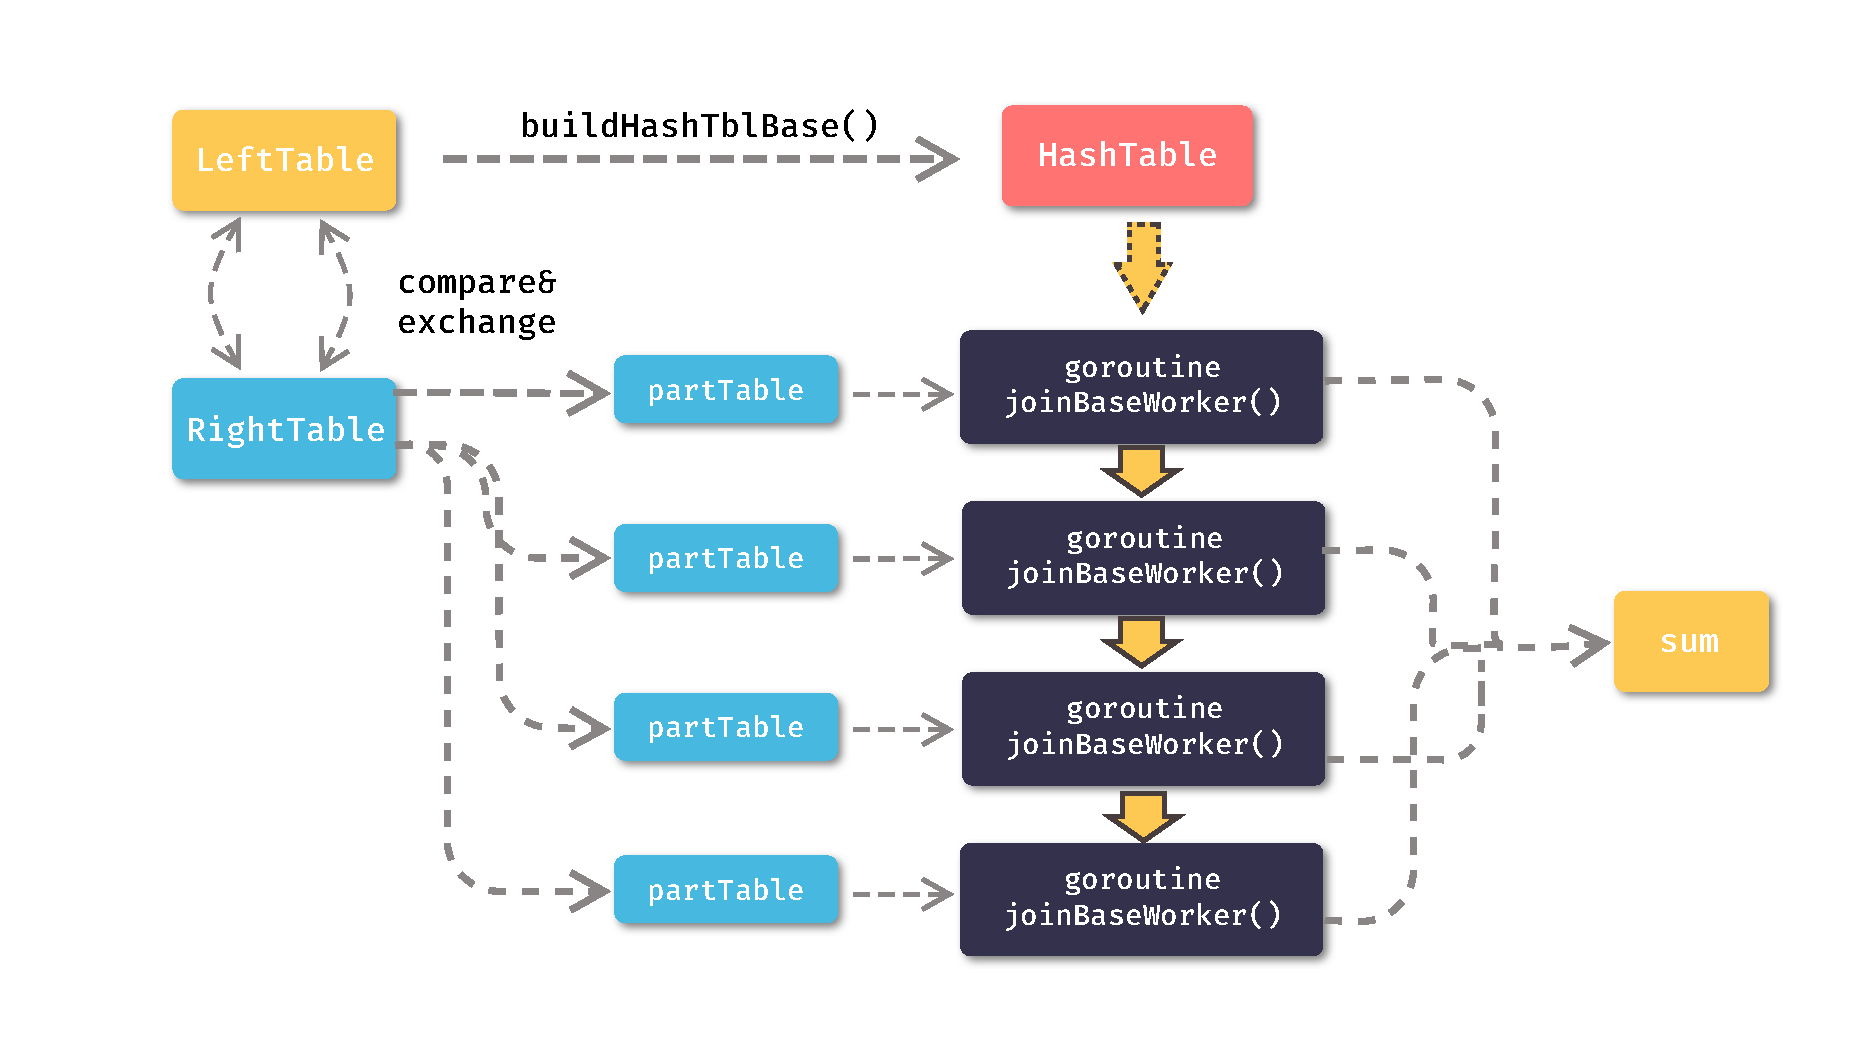
\includegraphics[width=0.9\textwidth]{fig/base.pdf}\\
  \caption{JoinBase}
  \label{joinbase}
\end{figure}

下面是实现$JoinBase$所用的主要代码,因为在当左表不是较小的那个表的时候,在对右表hash和使用左表进行probe的时候需要有不同的处理,
hash右表的时候键值对存储的一个数组,其中数组的长度代表右表中产生同一个hash值的个数数,在使用左表进行probe的时候,计算(左表匹配到的那一行的第0位值)*(从hash表读出数组的长度)。
下面的代码中会有相应的解释。
\begin{lstlisting}[language={Golang}]
  func buildHashTblBase(tbl [][]string, offset []int, flag bool) (hashtable *mvmap.MVMap){
    ...
    for _, row := range tbl {
      for j, off := range offset {
        if j > 0 {
          keyBuffer = append(keyBuffer, '_')
        }
        keyBuffer = append(keyBuffer, []byte(row[off])...)
      }
      switch flag {
      case true:
        // 当使用右表进行hash的时候,我们只要简单的向keyBuffer对应的值中插入一个大小为0的[]byte数组就行,因为这里值是用来存储数据长度的。
        hashtable.Put(keyBuffer, valBuffer)
      case false:
        // 当使用左表进行hash的时候,我们这里选择存储row[0]的值,在probe阶段就不用再去查找左表来计算sum值了。
        v, err := strconv.ParseInt(row[0], 10, 64)
        if err != nil {
          panic("hashWorker Convert\n" + err.Error())
        }
        *(*int64)(unsafe.Pointer(&valBuffer[0])) = int64(v)
        hashtable.Put(keyBuffer, valBuffer)
      }
      keyBuffer = keyBuffer[:0]
    }
    return
  }
\end{lstlisting}

\begin{lstlisting}[language={Golang}]
  func joinBaseWorker(hashtable *mvmap.MVMap, outerSlice [][]string, innertbl [][]string, offset []int, resultCh chan uint64, flag bool) {
    ...
    for _, row := range outerSlice {
      for i, off := range offset{
        if i > 0 {
          keyHash = append(keyHash, '_')
        }
        keyHash = append(keyHash, []byte(row[off])...)
      }
      vals = hashtable.Get(keyHash, vals)
      keyHash = keyHash[:0]
      switch flag {
      case true:
        // 当使用右表进行probe的时候,我们取出左表对应的row[0]值和从hash表中查找到的数组长度相乘,用来计算sum。
        v, err := strconv.ParseInt(row[0], 10, 64)
        if err != nil {
          panic("joinBaseWorker Convert\n" + err.Error())
        }
        t := v * int64(len(vals))
        sum += uint64(t)
      case false:
        // 当使用左表进行probe的时候,我们从hash表获取到相应的值之后进行累加进行就可以了。
        for _, val := range vals {
          v := *(*int64)(unsafe.Pointer(&val[0]))
          sum += uint64(v)
        }
      }
      vals = vals[:0]
    }
    resultCh <- sum
  }
\end{lstlisting}

\subsubsection{$JoinBase$的性能分析}
通过2.1的实验结果可以看到在数据量较小的时候,和$JoinExample$相比性能优化了30\%左右,
在数据量较大的情况下,也能够优化30\%左右。其中我们注意到,当左表大于右表的情况下,$JoinExample$
会受到影响,执行较慢。而$JoinBase$执行时间不会受到影响。因为对小表做hash操作,并对大表hash处理,
能够起到较好的优化效果。

我们使用pprof查看性能瓶颈出现在哪里。

\begin{lstlisting}[language={bash}]
  go tool pprof cpu.prof                                                                                                      ─╯
  Type: cpu
  Time: Feb 26, 2020 at 2:06pm (CST)
  Duration: 7.59s, Total samples = 11.58s (152.48%)
  Entering interactive mode (type "help" for commands, "o" for options)
  (pprof) top
  Showing nodes accounting for 7990ms, 69.00% of 11580ms total
  Dropped 77 nodes (cum <= 57.90ms)
  Showing top 10 nodes out of 102
        flat  flat%   sum%        cum   cum%
      1520ms 13.13% 13.13%     1520ms 13.13%  syscall.syscall
      1490ms 12.87% 25.99%     1490ms 12.87%  runtime.memmove
      1460ms 12.61% 38.60%     3810ms 32.90%  runtime.scanobject
       690ms  5.96% 44.56%     4010ms 34.63%  join.readCSVFileIntoTbl
       690ms  5.96% 50.52%      760ms  6.56%  runtime.mapaccess1_fast64
       550ms  4.75% 55.27%     1140ms  9.84%  runtime.findObject
       480ms  4.15% 59.41%      510ms  4.40%  runtime.spanOf
       470ms  4.06% 63.47%      470ms  4.06%  runtime.madvise
       320ms  2.76% 66.23%     2300ms 19.86%  encoding/csv.(*Reader).readRecord
       320ms  2.76% 69.00%      320ms  2.76%  runtime.memclrNoHeapPointers
\end{lstlisting}

通过top指令我们可以看到函数readCSVFileIntoTbl运行时间占据了大部分,除此之外函数scanobject代表golang
在进行垃圾回收时候进行对象扫描时候的费时,而我们编写的函数并没有列出来,说明主要的问题还是IO,而且一次读入大量的
数据,也会造成gc压力。接着用pprof对内存进行分析,通过图\ref{joinbase-mem}我们看到在文件读取中确实申请了
大量内存,导致gc压力过大。

\begin{figure}[H]
  \centering
  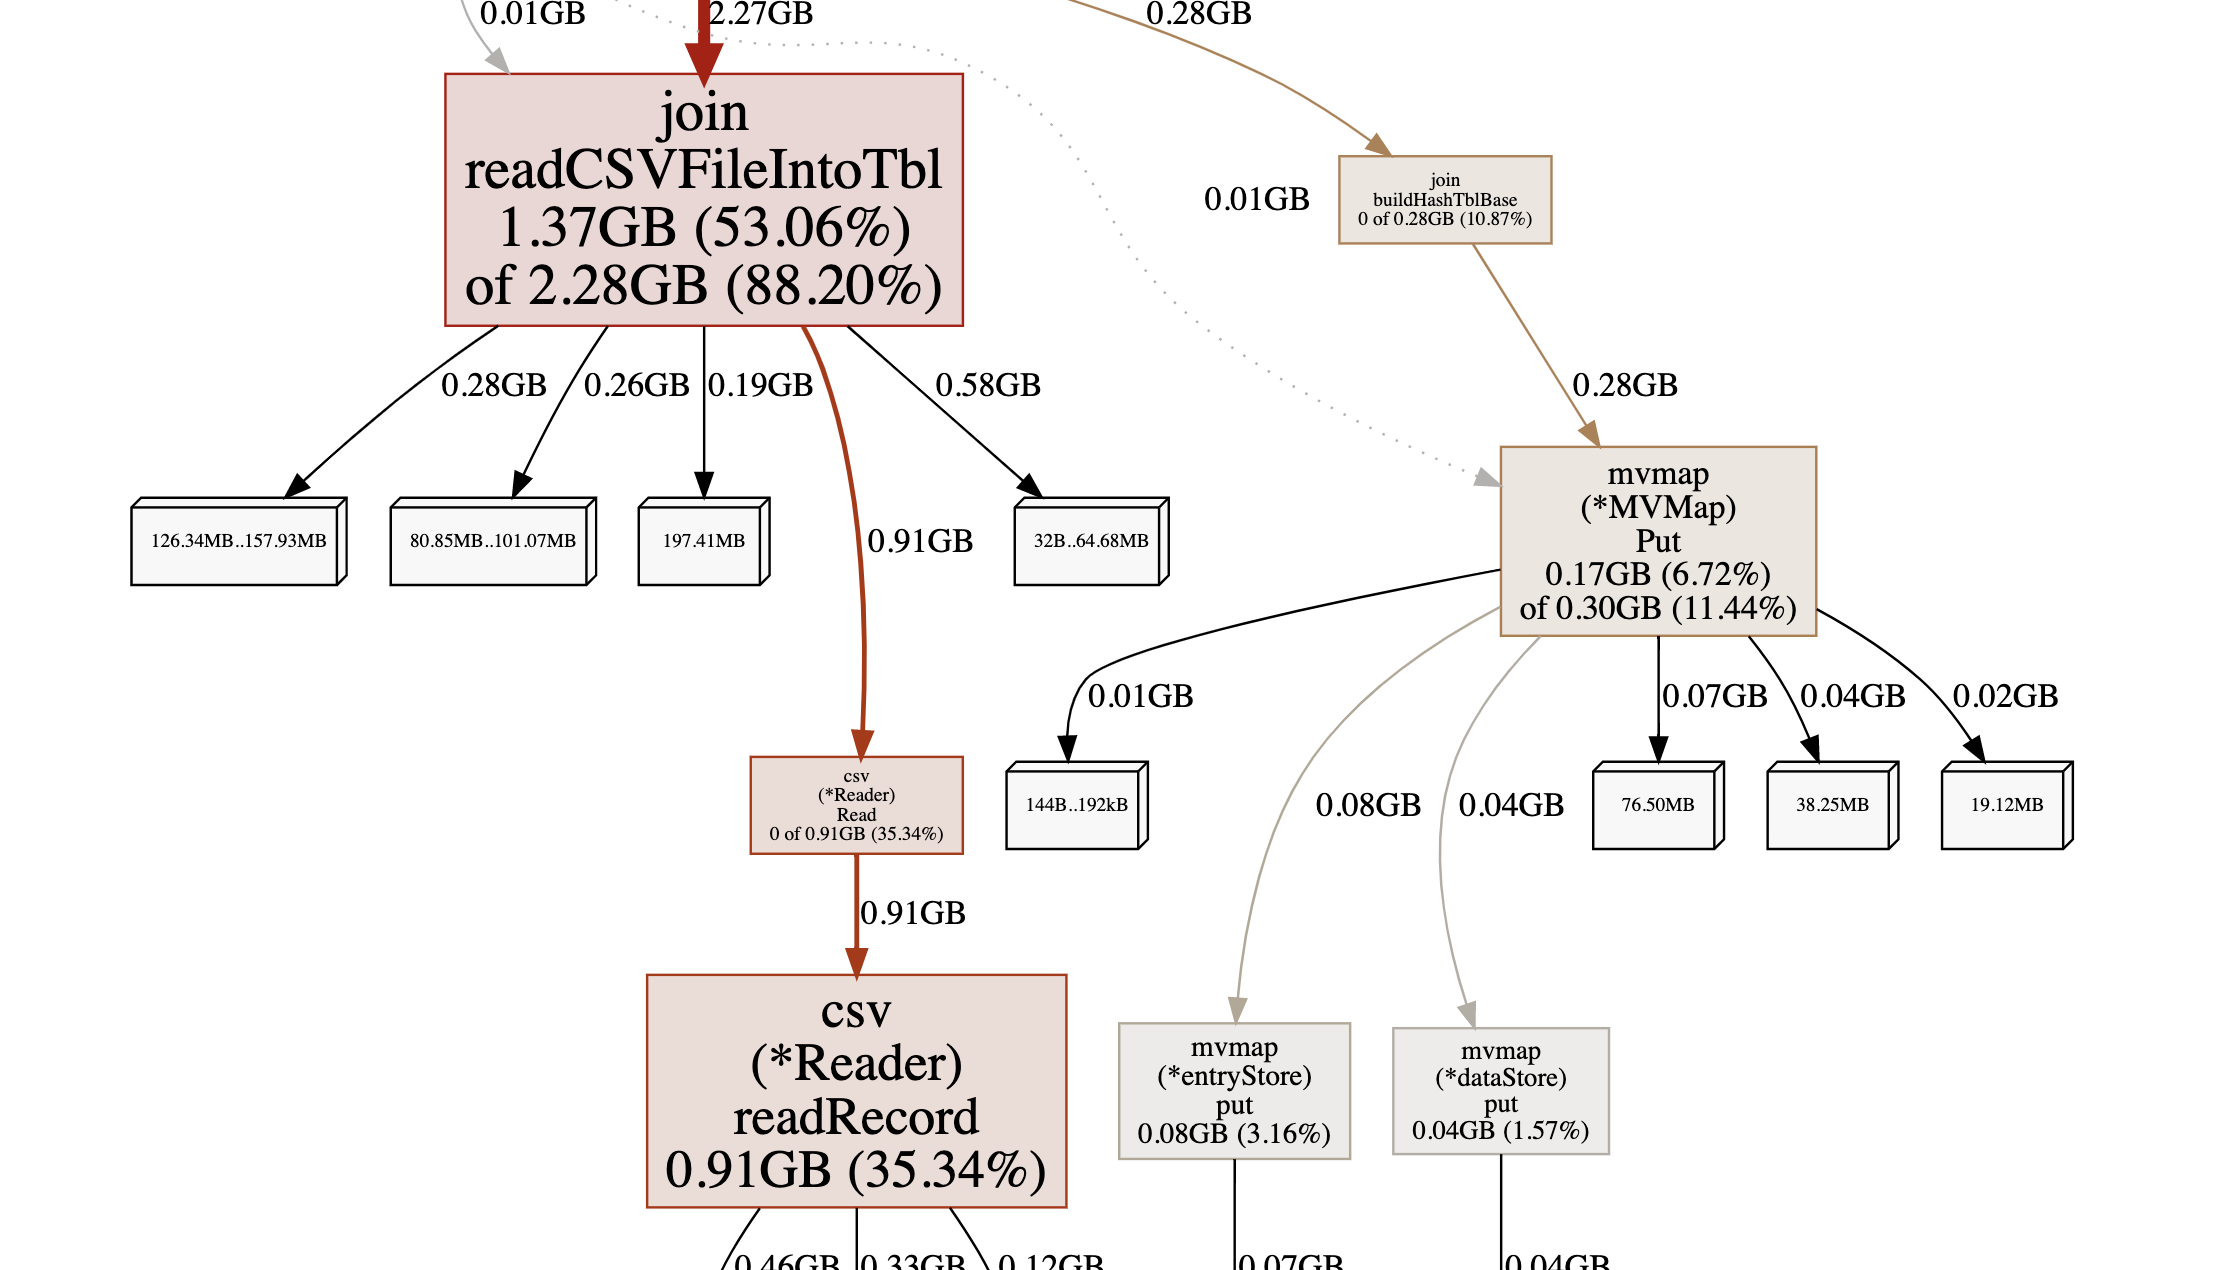
\includegraphics[width=0.9\textwidth]{fig/base-mem.png}\\
  \caption{JoinBase-MEM}
  \label{joinbase-mem}
\end{figure}

\subsubsection{IO/CPU交叠执行的$Join$}
和做section2时候出现的问题一样,代码执行的主要瓶颈还是磁盘IO和gc,一次性读入内存大量的数据,给系统gc也带来了
很大的压力,为了解决这种问题,本节的解决方案是用一个goroutine A分块读入数据,然后将数据块通过管道传递给另一个goroutine B
数据进行hash和probe。然后A接着读入数据直到数据读入结束。但是因为IO读取速度过于缓慢,远不及CPU的处理速度,所以
暂时没有想到能够用到多核资源的方法,只能一个goroutine读取数据,一个goroutine进行数据处理。部分代码如下,下面展示的代码是分块读取数据部分,
hash和probe部分和上面的代码类似,就不赘述了。

\begin{figure}[H]
  \centering
  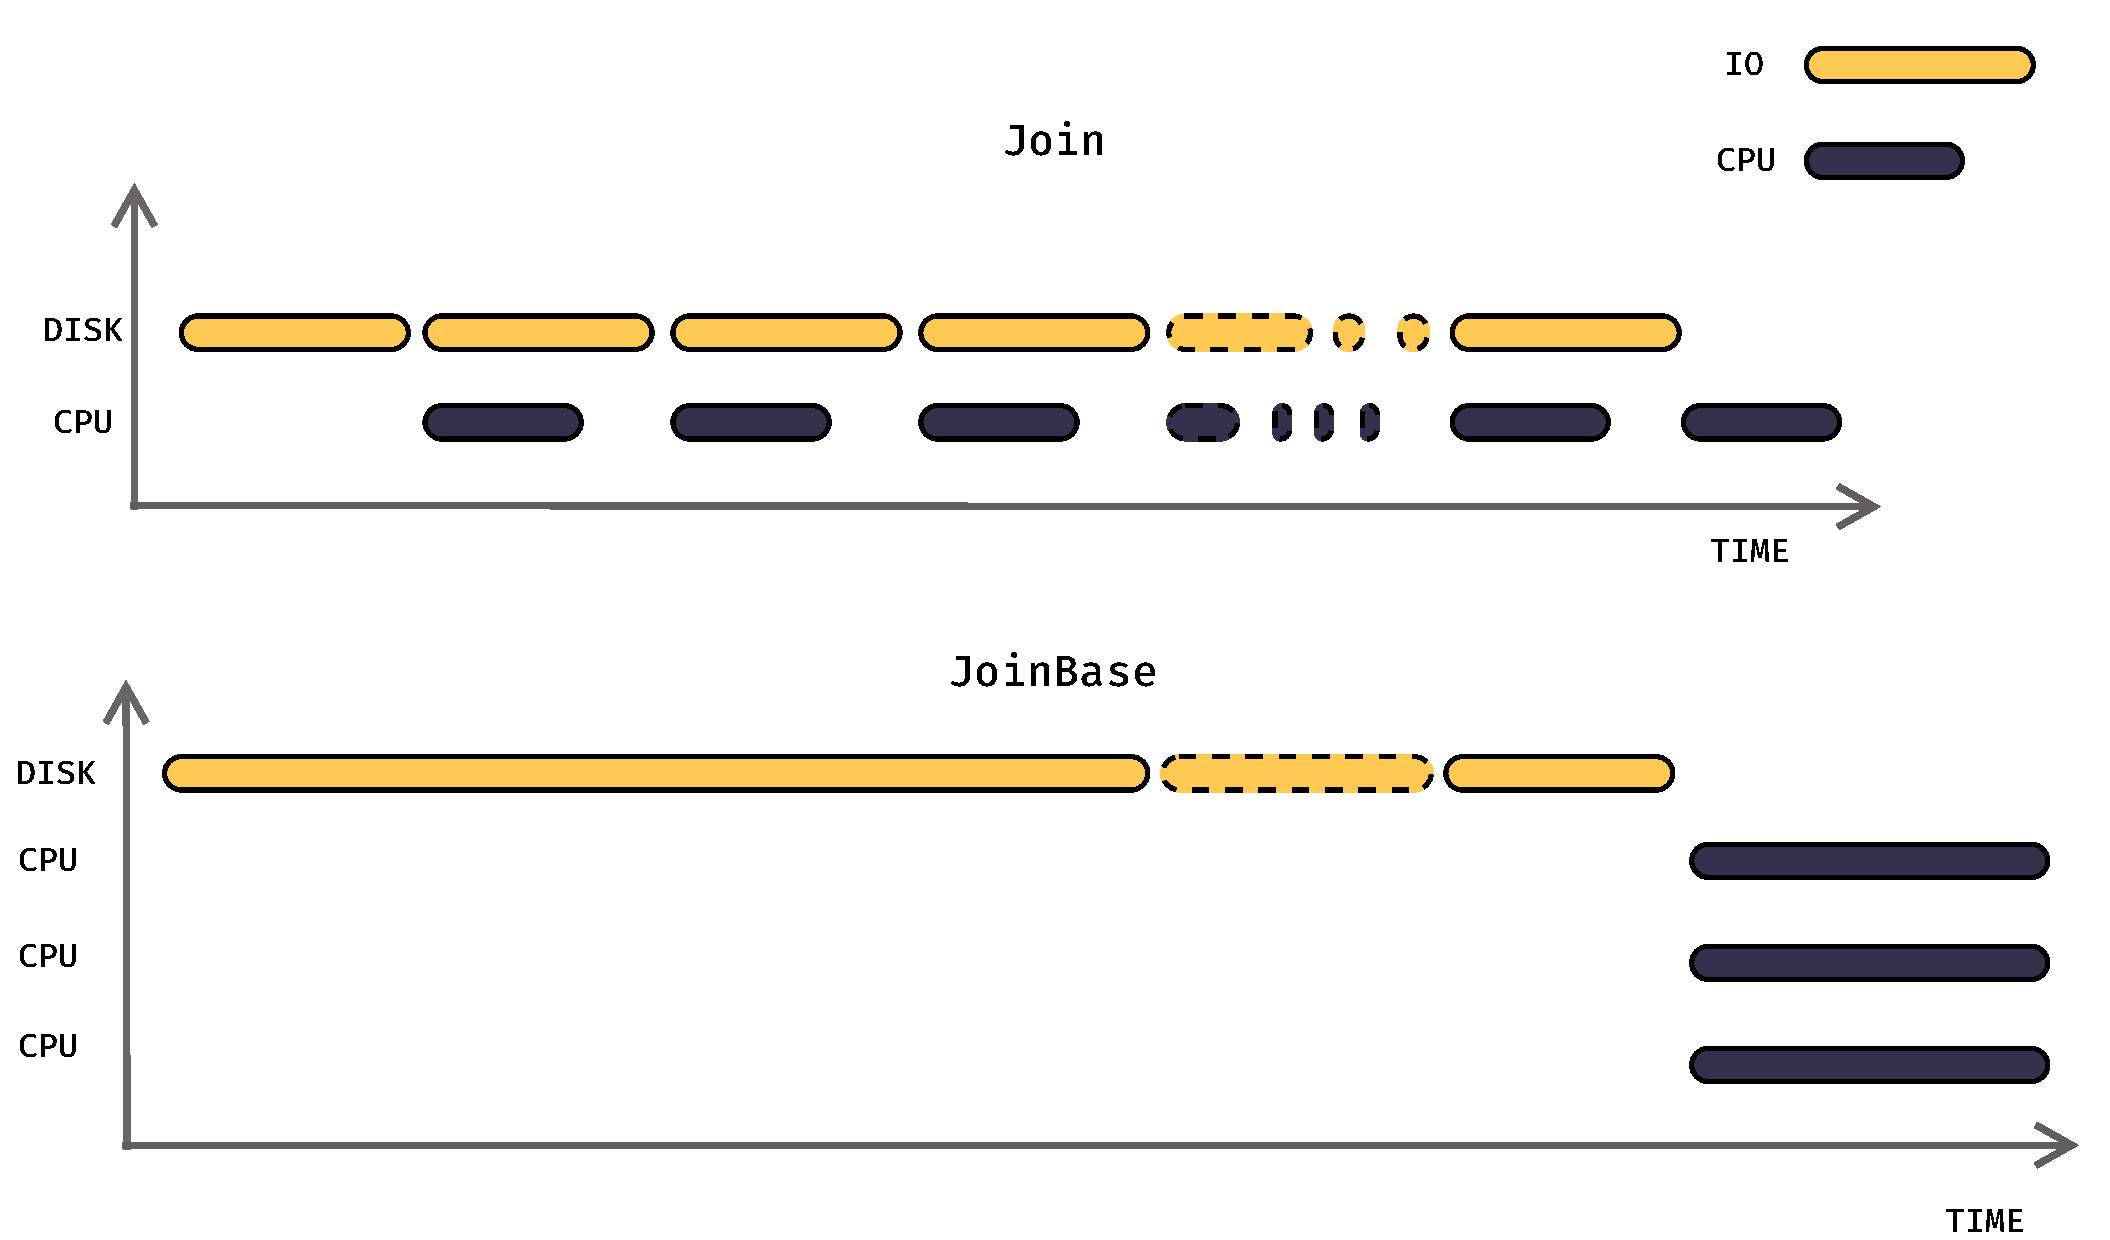
\includegraphics[width=0.7\textwidth]{fig/io.pdf}\\
  \caption{JoinBase}
  \label{join}
\end{figure}

\begin{lstlisting}[language={Golang}]
func fecthCSVBlock(f string, blockResourceCh chan [][]string){
	defer close(blockResourceCh)
  ... 
	csvReader := csv.NewReader(csvFile)
	block := make([][]string, 0, blockLine)
	c := 0
	for {
		row, err := csvReader.Read()
		if err == io.EOF {
			break
		} else if err != nil {
			panic("ReadCSVFile " + f + "fail\n" + err.Error())
		}
		c++
    block = append(block, row)
    // 当从磁盘读入一个block块的数据之后,将数据传递给通道,hashWork会读取block的数据进行数据处理。
		if c == blockLine {
			blockResourceCh <- block
			c = 0
			block = make([][]string, 0, blockLine)
		}
	}
	blockResourceCh <- block
}
\end{lstlisting}

如图\ref{join}所示,我们分块对数据读取,只要保证每次读数据块的时间大于cpu对数据处理的时间即可,和$JoinBase$
全部读取相比,能够较好的利用从磁盘读入数据这段时间,算法大概的流程如下:

\begin{enumerate}
  \item 分块读取左表的数据,将block传递给hashWork进行hash产生hash表
  \item 接着分块读取右表的数据,将数据块传递给joinWorker进行join操作,并计算sum值。
\end{enumerate}


\subsubsection{$Join$的性能分析}

通过2.1的实验结果对比,在小数据量的情况下,Join性能优化了36\%左右,而在较大数据情况下,
性能优化了55\%左右。

我们对程序进行pprof分析,通过对CPU进行分析,虽然IO相关函数执行时间还是最长,因为这是避免不了的,
但是gc相关的函数执行时间大大降低,说明分块读取确实降低了gc的压力;除此之外,函数$runtime.pthread\_cond\_wait$
的执行时间较大,因为我们的cpu处理时间大大大于IO读取,所以worker一定会去等待数据块的到来,就造成了
通道等待。

\begin{lstlisting}[language={bash}]
  Showing nodes accounting for 4940ms, 93.21% of 5300ms total
  Dropped 32 nodes (cum <= 26.50ms)
  Showing top 10 nodes out of 67
        flat  flat%   sum%        cum   cum%
      2130ms 40.19% 40.19%     2130ms 40.19%  syscall.syscall
      1300ms 24.53% 64.72%     1300ms 24.53%  runtime.pthread_cond_wait
       350ms  6.60% 71.32%      350ms  6.60%  runtime.madvise
       270ms  5.09% 76.42%      270ms  5.09%  github.com/pingcap/tidb/util/mvmap.(*entryStore).put
       240ms  4.53% 80.94%      240ms  4.53%  runtime.pthread_cond_signal
       180ms  3.40% 84.34%      180ms  3.40%  runtime.(*bmap).overflow
       130ms  2.45% 86.79%     2320ms 43.77%  encoding/csv.(*Reader).readRecord
       120ms  2.26% 89.06%      160ms  3.02%  runtime.evacuate_fast64
       110ms  2.08% 91.13%      110ms  2.08%  runtime.mapaccess1_fast64
       110ms  2.08% 93.21%      110ms  2.08%  runtime.usleep
\end{lstlisting}

\subsection{总结}
总的来说,目前能做到的只能通过分块读取来加速计算了,一开始想到的是多线程优化,后来经过
同学指点,采取了第二个方式进行优化,优化效果基本上就这样了。

这是最后一个section,通过4个section的学习,学到了很多关于数据库和分布式的知识,
而且多数的性能优化和自己最开始想的不一样,但是最后发现最大的优化层面都在IO层面优化,
因为本人的文字描述水平有限,所以就画了一些图片来更加形象的描述。

\end{document}
